\section{Исследовательский раздел}

В данном разделе будет приведено описание исследования зависимости времени ответа от количества запросов в секунду и сравнения эффективности реализаций приложения с использованием дополнительного кеширования и без него, технические характеристики устройства, на котором оно проводилось, и представлены его результаты.

% \subsection*{Цель исследования}

% Целью исследования является получение зависимости времени ответа от количества запросов в секунду и сравнения эффективности реализаций приложения с использованием дополнительного кеширования и без него.

\subsection{Описание исследования}

В качестве базы данных для дополнительного кеширования была выбрана KeyDB~\cite{keydb}, так как ее функциональности достаточно для обеспечения кеширования, а также она является бесплатной и открытой альтернативой Redis~\cite{redis} --- известной базы данных для этих целей~\cite{redis-jobs}.

В качестве инструмента для проведения нагрузочного тестирования был выбран Locust~\cite{locust}, так как его функциональности достаточно для проведения нагрузочного тестирования, а также присутствует возможность написания тестовых сценариев на простом скриптовом языке Python~\cite{python}.

Проведение нагрузочного тестирования в Locust состоит из нескольких этапов:
\begin{enumerate}
    \item Написание сценариев тестирования в файле locustfile.py;
    \item Установка максимального количества запросов в секунду, шага увеличения количества запросов в секунду и времени, на протяжении которого будет проводиться нагрузочного тестирования;
    \item Просмотр и экспорт статистики и результатов проведенного нагрузочного тестирования.
\end{enumerate}

Содержимое файла со сценариями тестирования приведено в листинге \ref{lst:locustfile} приложения А; пример использования кеша в приложении --- в листинге \ref{lst:go:cache}, а примеры интерфейса Locust, соответствующие этапам 2 и 3 проведения нагрузочного тестирования --- на рисунках \ref{locust:1} -- \ref{locust:3} ниже.

\begin{figure}[H]
	\centering
	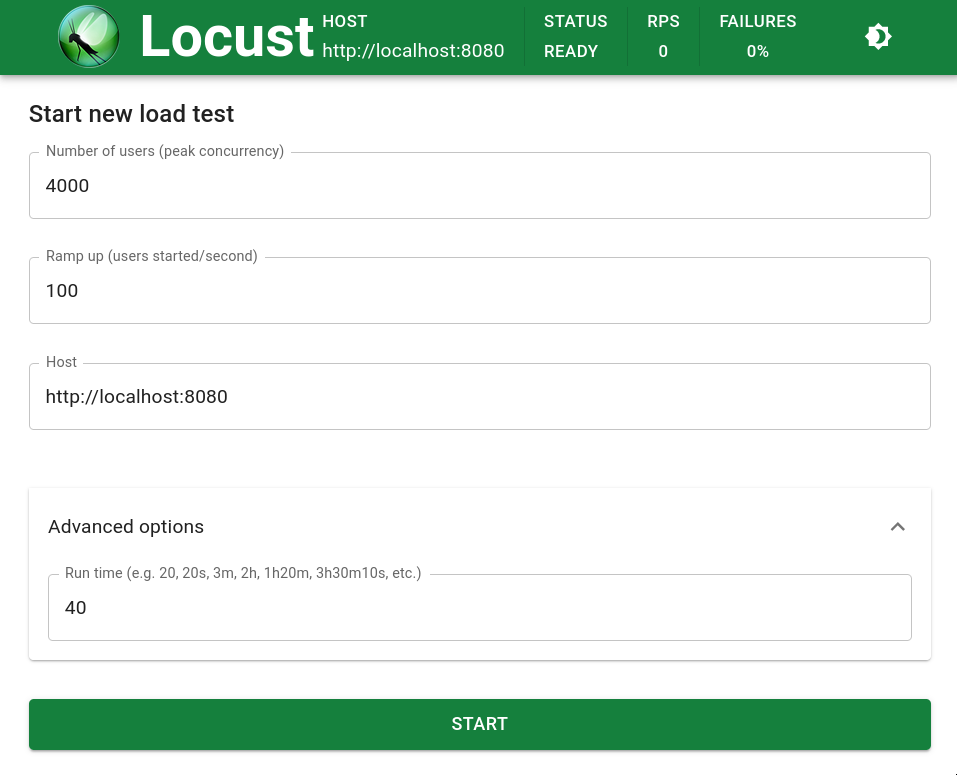
\includegraphics[width=0.9\textwidth]{img/locust-scr-1.png}
	\caption{Запуск нагрузочного тестирования в Locust}
	\label{locust:1}
\end{figure}

\begin{figure}[H]
	\centering
	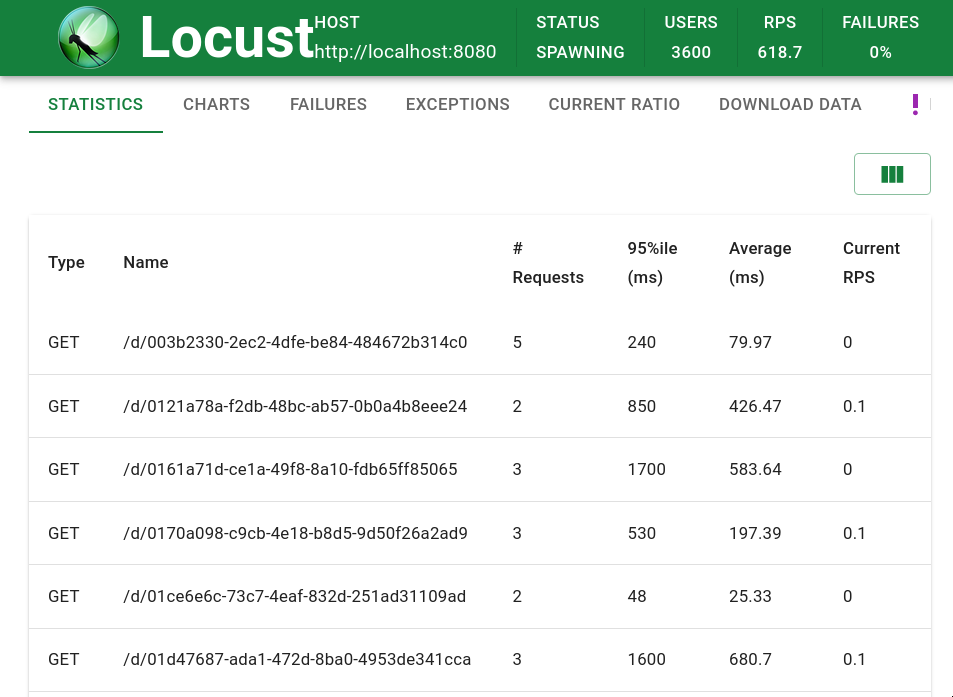
\includegraphics[width=0.9\textwidth]{img/locust-scr-2.png}
	\caption{Просмотр статистики нагрузочного тестирования в реальном времени}
	\label{locust:2}
\end{figure}

\begin{figure}[H]
	\centering
	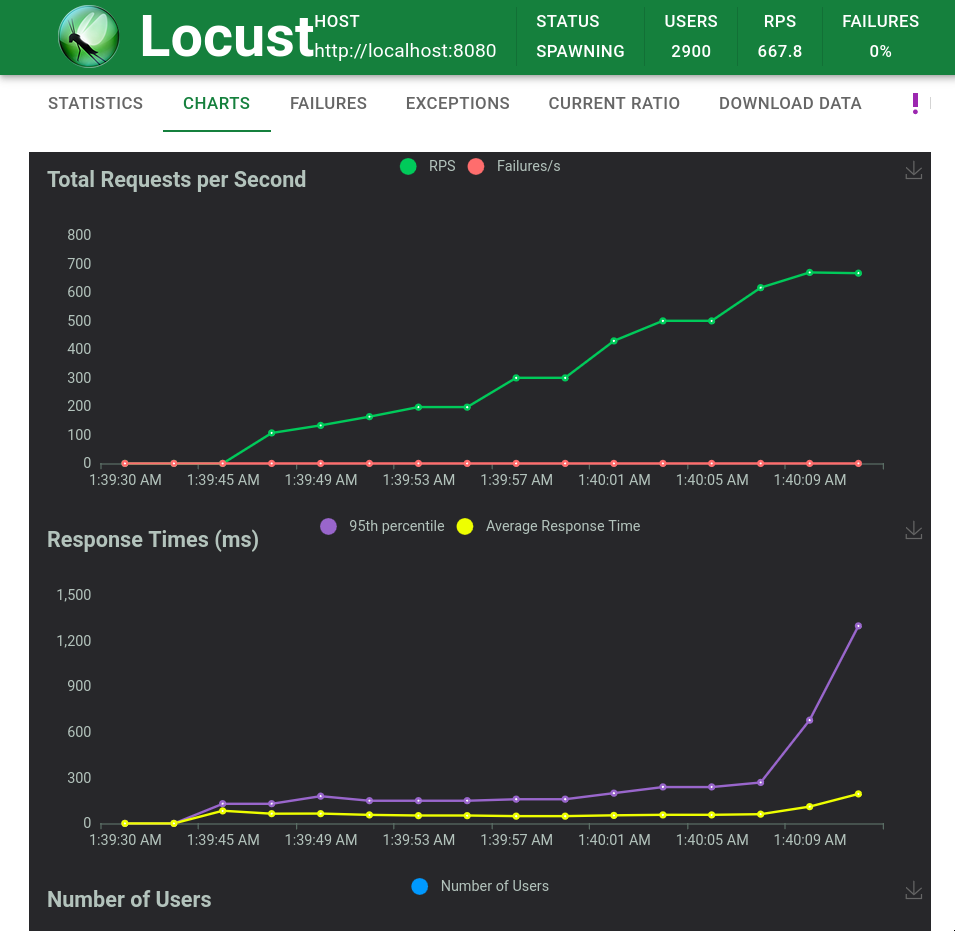
\includegraphics[width=0.9\textwidth]{img/locust-scr-3.png}
	\caption{Просмотр графиков нагрузочного тестирования в реальном времени}
	\label{locust:3}
\end{figure}

\newpage

\subsection{Технические характеристики}

Технические характеристики устройства, на котором выполнялись замеры времени, представлены ниже.
\begin{enumerate}
    \item Процессор: \texttt{AMD Ryzen 7 4700U} 2.0 ГГц~\cite{amd}, 8 физических ядер, 8 потоков;
    \item Оперативная память: 8 ГБ, \texttt{DDR4}, 3200 МГц;
    \item Операционная система: \texttt{NixOS 23.11.1209.933d7}~\cite{nixos};
    \item Версия ядра: \texttt{6.1.64}.
\end{enumerate}

При выполнении замеров времени ноутбук был подключен к сети электропитания, был запущен браузер Chromium~\cite{chromium} с одной вкладкой, три терминала Alacritty~\cite{alacritty}, в которых выполнялись Locust, сервер на Go и Neovim.
На фоне работал Docker-контейнер~\cite{docker} с базой данных.

\subsection{Результаты исследования}

Далее приведены таблицы и графики с результатами исследования.
Поясняющие комментарии к таблицам приводятся после таблицы \ref{tab:cache:95}; к графикам --- после каждого графика.

Данные в правых колонках таблиц являются усредненным значением из общего количества запросов к моменту времени, когда число запросов в секунду составляло значение из левой колонки таблицы.
Так, например, в таблице \ref{tab:nocache:avg} время ответа 0.086 секунд является средним из 10 запросов, а время ответа 0.555 секунд --- средним из 15438 запросов, так как нагрузочное тестирование проводилось на протяжении 40 секунд с приростом количества имитируемых пользователей приложения --- 100 новых пользователей в секунду.
В таблице \ref{tab:cache:avg} время ответа 0.465 является средним из  16103 запросов.

\begin{table}[H]
\centering
\caption{Зависимость среднего времени ответа от количества запросов в секунду без использования кеширования}
% \begin{tabular}{|c|c|}
% \begin{tabular}{|m{8cm}|m{8cm}|}
\begin{tabular}{|m{6.85cm}|m{9.25cm}|}
\hline
    \,\hfill \textbf{Число запросов в секунду} & \,\hfill \textbf{Среднее время ответа (с)} \hfill\, \\ \hline
    \,\hfill 10 \hfill\, & \,\hfill 0.086 \hfill\, \\ \hline
    \,\hfill 27 \hfill\, & \,\hfill 0.068 \hfill\, \\ \hline
    \,\hfill 61 \hfill\, & \,\hfill 0.058 \hfill\, \\ \hline
    \,\hfill 93 \hfill\, & \,\hfill 0.060 \hfill\, \\ \hline
    \,\hfill 25 \hfill\, & \,\hfill 0.050 \hfill\, \\ \hline
    \,\hfill 87 \hfill\, & \,\hfill 0.044 \hfill\, \\ \hline
    \,\hfill 56 \hfill\, & \,\hfill 0.047 \hfill\, \\ \hline
    \,\hfill 81 \hfill\, & \,\hfill 0.055 \hfill\, \\ \hline
    \,\hfill 44 \hfill\, & \,\hfill 0.070 \hfill\, \\ \hline
    \,\hfill 96 \hfill\, & \,\hfill 0.095 \hfill\, \\ \hline
    \,\hfill 22 \hfill\, & \,\hfill 0.222 \hfill\, \\ \hline
    \,\hfill 27 \hfill\, & \,\hfill 0.290 \hfill\, \\ \hline
    \,\hfill 41 \hfill\, & \,\hfill 0.465 \hfill\, \\ \hline
    \,\hfill 52 \hfill\, & \,\hfill 0.555 \hfill\, \\ \hline
\end{tabular}
\label{tab:nocache:avg}
\end{table}

\begin{table}[H]
\centering
\caption{Зависимость 95-го процентиля времени ответа от количества запросов в секунду без использования кеширования}
% \begin{tabular}{|c|c|}
% \begin{tabular}{|m{8cm}|m{8cm}|}
\begin{tabular}{|m{6.85cm}|m{9.25cm}|}
\hline
    % \,\hfill \textbf{Число запросов в секунду} \hfill\, & \,\hfill \textbf{95-й процентиль времени ответа (с)} \hfill\, \\ \hline
    \,\hfill \textbf{Число запросов в секунду} & \,\hfill \textbf{95-й процентиль времени ответа (с)} \\ \hline
    \,\hfill  10 \hfill\, & \,\hfill 0.110 \hfill\, \\ \hline
    \,\hfill 127 \hfill\, & \,\hfill 0.160 \hfill\, \\ \hline
    \,\hfill 161 \hfill\, & \,\hfill 0.150 \hfill\, \\ \hline
    \,\hfill 193 \hfill\, & \,\hfill 0.180 \hfill\, \\ \hline
    \,\hfill 225 \hfill\, & \,\hfill 0.160 \hfill\, \\ \hline
    \,\hfill 387 \hfill\, & \,\hfill 0.160 \hfill\, \\ \hline
    \,\hfill 456 \hfill\, & \,\hfill 0.170 \hfill\, \\ \hline
    \,\hfill 581 \hfill\, & \,\hfill 0.260 \hfill\, \\ \hline
    \,\hfill 644 \hfill\, & \,\hfill 0.330 \hfill\, \\ \hline
    \,\hfill 696 \hfill\, & \,\hfill 0.450 \hfill\, \\ \hline
    \,\hfill 722 \hfill\, & \,\hfill 1.200 \hfill\, \\ \hline
    \,\hfill 727 \hfill\, & \,\hfill 1.600 \hfill\, \\ \hline
    \,\hfill 741 \hfill\, & \,\hfill 2.800 \hfill\, \\ \hline
    \,\hfill 752 \hfill\, & \,\hfill 3.800 \hfill\, \\ \hline
\end{tabular}
\label{tab:nocache:95}
\end{table}

\begin{table}[H]
\centering
\caption{Зависимость среднего времени ответа от количества запросов в секунду при использовании кеширования}
% \begin{tabular}{|c|c|}
% \begin{tabular}{|m{8cm}|m{8cm}|}
\begin{tabular}{|m{6.85cm}|m{9.25cm}|}
\hline
    % \,\hfill \textbf{Число запросов в секунду} \hfill\, & \,\hfill \textbf{Среднее время ответа (с)} \hfill\, \\ \hline
    \,\hfill \textbf{Число запросов в секунду} & \,\hfill \textbf{Среднее время ответа (с)} \hfill\, \\ \hline
    \,\hfill  10 \hfill\, & \,\hfill 0.086 \hfill\, \\ \hline
    \,\hfill 112 \hfill\, & \,\hfill 0.070 \hfill\, \\ \hline
    \,\hfill 172 \hfill\, & \,\hfill 0.063 \hfill\, \\ \hline
    \,\hfill 202 \hfill\, & \,\hfill 0.060 \hfill\, \\ \hline
    \,\hfill 236 \hfill\, & \,\hfill 0.053 \hfill\, \\ \hline
    \,\hfill 300 \hfill\, & \,\hfill 0.050 \hfill\, \\ \hline
    \,\hfill 362 \hfill\, & \,\hfill 0.049 \hfill\, \\ \hline
    \,\hfill 424 \hfill\, & \,\hfill 0.050 \hfill\, \\ \hline
    \,\hfill 493 \hfill\, & \,\hfill 0.054 \hfill\, \\ \hline
    \,\hfill 611 \hfill\, & \,\hfill 0.058 \hfill\, \\ \hline
    \,\hfill 685 \hfill\, & \,\hfill 0.074 \hfill\, \\ \hline
    \,\hfill 730 \hfill\, & \,\hfill 0.110 \hfill\, \\ \hline
    \,\hfill 761 \hfill\, & \,\hfill 0.238 \hfill\, \\ \hline
    \,\hfill 771 \hfill\, & \,\hfill 0.303 \hfill\, \\ \hline
    \,\hfill 780 \hfill\, & \,\hfill 0.465 \hfill\, \\ \hline
\end{tabular}
\label{tab:cache:avg}
\end{table}

\begin{table}[H]
\centering
\caption{Зависимость 95-го процентиля времени ответа от количества запросов в секунду при использовании кеширования}
% \begin{tabular}{|c|c|}
\begin{tabular}{|m{6.85cm}|m{9.25cm}|}
\hline
    \,\hfill \textbf{Число запросов в секунду} & \,\hfill \textbf{95-й процентиль времени ответа (с)} \\ \hline
    \,\hfill  10 \hfill\, & \,\hfill 0.130 \hfill\, \\ \hline
    \,\hfill 112 \hfill\, & \,\hfill 0.120 \hfill\, \\ \hline
    \,\hfill 172 \hfill\, & \,\hfill 0.170 \hfill\, \\ \hline
    \,\hfill 202 \hfill\, & \,\hfill 0.180 \hfill\, \\ \hline
    \,\hfill 236 \hfill\, & \,\hfill 0.170 \hfill\, \\ \hline
    \,\hfill 300 \hfill\, & \,\hfill 0.170 \hfill\, \\ \hline
    \,\hfill 362 \hfill\, & \,\hfill 0.180 \hfill\, \\ \hline
    \,\hfill 424 \hfill\, & \,\hfill 0.180 \hfill\, \\ \hline
    \,\hfill 493 \hfill\, & \,\hfill 0.210 \hfill\, \\ \hline
    \,\hfill 611 \hfill\, & \,\hfill 0.250 \hfill\, \\ \hline
    \,\hfill 685 \hfill\, & \,\hfill 0.320 \hfill\, \\ \hline
    \,\hfill 730 \hfill\, & \,\hfill 0.470 \hfill\, \\ \hline
    \,\hfill 761 \hfill\, & \,\hfill 1.300 \hfill\, \\ \hline
    \,\hfill 771 \hfill\, & \,\hfill 1.500 \hfill\, \\ \hline
    \,\hfill 780 \hfill\, & \,\hfill 3.100 \hfill\, \\ \hline
\end{tabular}
\label{tab:cache:95}
\end{table}

По таблицам \ref{tab:nocache:avg} и \ref{tab:cache:avg} можно увидеть, что при 752 запросах в секунду к приложению, не использующему кеш KeyDB, среднее время ответа составляет 0.555 секунд, а при 780 запросах в секунду к приложению, использующему кеш KeyDB, среднее время ответа составляет 0.465 секунд.

По таблицам \ref{tab:nocache:95} и \ref{tab:cache:95} можно увидеть, что 95 процентов запросов при 752 запросах в секунду к приложению, не использующему кеш KeyDB, обрабатываются быстрее 3.8 секунд, а при 780 запросах в секунду к приложению, использующему кеш KeyDB, 95 процентов запросов обрабатываются быстрее 3.1 секунды.

\begin{figure}[H]
	\centering
	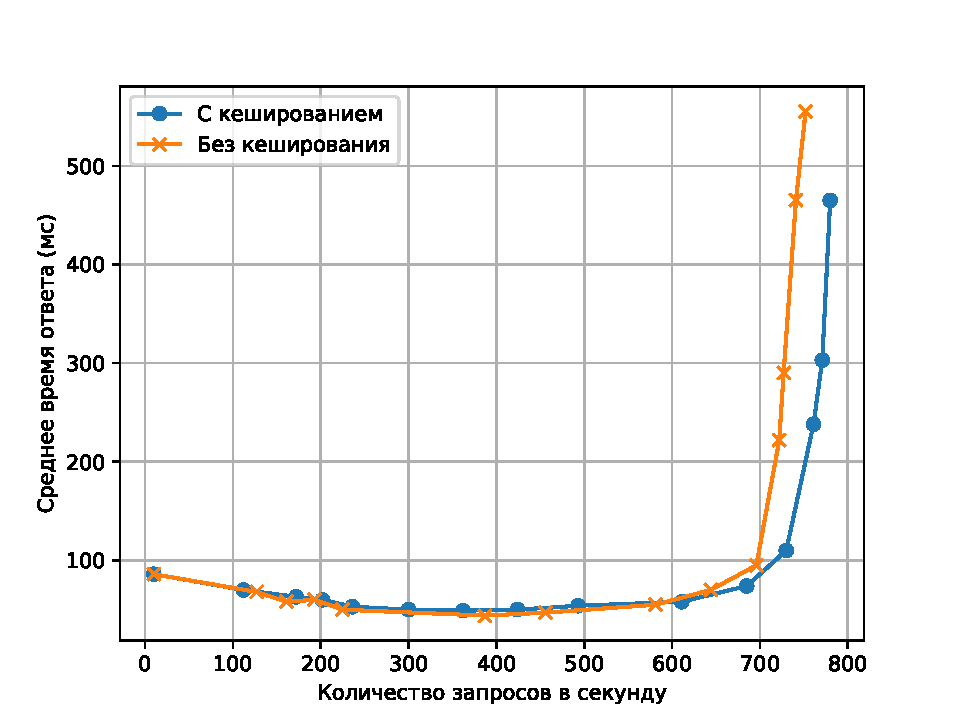
\includegraphics[width=0.9\textwidth]{img/avg-resp-time.pdf}
	\caption{Зависимость среднего времени ответа от количества запросов в секунду}
	\label{plot:avg}
\end{figure}

По графику \ref{plot:avg} можно заметить, что среднее время ответа убывает примерно до 350 запросов в секунду, после чего начинается экспоненциальный рост.
Более высокие значения среднего времени ответа на ранних этапах обусловлены тем, что большая часть запрашиваемых данных пока еще не находится в кеше KeyDB или базы данных.
После 600 запросов в секунду использование кеша KeyDB начинает давать прирост производительности.
При 730 запросах в секунду запросы к приложению, использующему кеш KeyDB, обрабатываются быстрее примерно в 2.64 раза.


\begin{figure}[H]
	\centering
	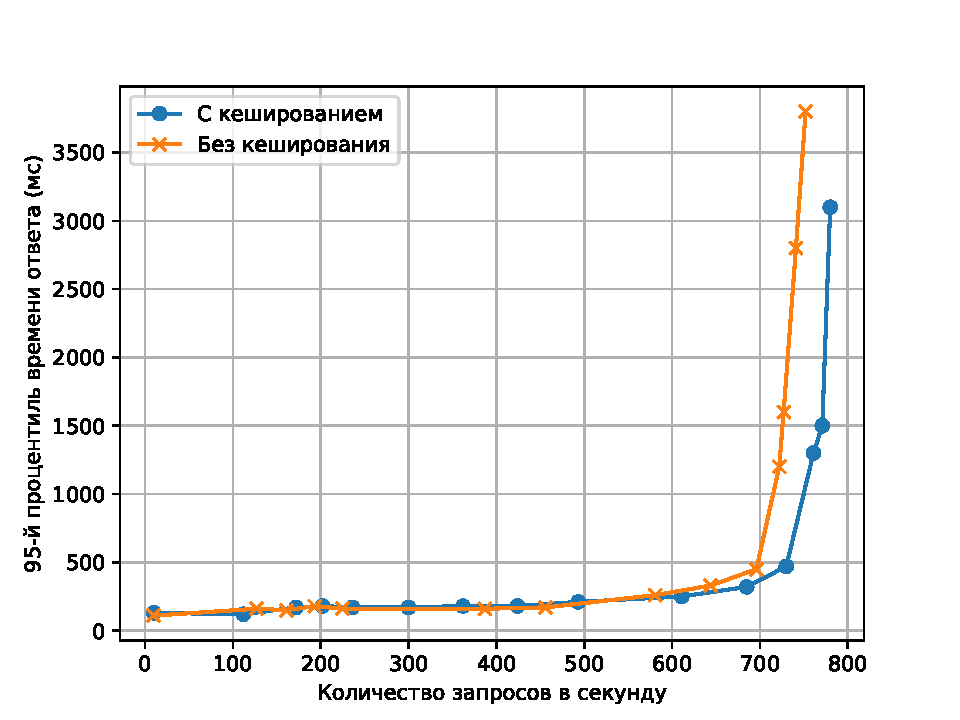
\includegraphics[width=0.9\textwidth]{img/95-resp-time.pdf}
	\caption{Зависимость 95-го процентиля времени ответа от количества запросов в секунду}
	\label{plot:95}
\end{figure}

По графику \ref{plot:95} видно, что при 750 запросах в секунду 95 процентов запросов к приложению, использующему кеш KeyDB, обрабатываются примерно в 3.45 раза быстрее.
После 700 запросов в секунду возникает резкий скачок 95-го процентили времени ответа и начинается экспоненциальный рост.

\subsection*{Вывод}

В данном разделе было проведено исследование зависимости времени ответа от количества запросов в секунду.
Среднее время ответа увеличивается с увеличением количества запросов в секунду.
В определенный момент среднее время ответа возрастает в 1.91 раз с увеличением количества запросов в секунду в 1.05 раза.

Использование дополнительного кеша позволяет ускорить среднее время ответа.
Так при 752 запросах в секунду использование кеша позволило ускорить среднее время ответа более, чем в 3 раза.
